%%%%%%%%%%%%%%%%%%%%%%%%%%%%%%%%%%%%%%%%%%%%%%%%%%%%%%%%%%%%%%%%%%%%%%%%%%%%%%%
% Titel:   Bericht - Pflichtenheft
% Autor:   gross10
% Datum:   13.12.2013
% Version: 0.0.1
%%%%%%%%%%%%%%%%%%%%%%%%%%%%%%%%%%%%%%%%%%%%%%%%%%%%%%%%%%%%%%%%%%%%%%%%%%%%%%%
%
%:::Change-Log:::
% Versionierung erfolgt auf folgende Gegebenheiten: -1. Release Versionen
%                                                   -2. Neue Kapitel
%                                                   -3. Fehlerkorrekturen
%
% 0.0.01      Erstellung der Datei
%%%%%%%%%%%%%%%%%%%%%%%%%%%%%%%%%%%%%%%%%%%%%%%%%%%%%%%%%%%%%%%%%%%%%%%%%%%%%%% 
\chapter{CAN Summary}\label{ch:can_summary}
	F�r die beiden Subteams Antrieb und Navigation wurde w�hrend der \gls{ac:pa2} ein Dokument zum CAN-Gatekeeper und seinen Funktionen erstellt. Die Unterlagen wurden laufend erg�ntzt und entsprechen dem aktuellen Stand der Dinge.
	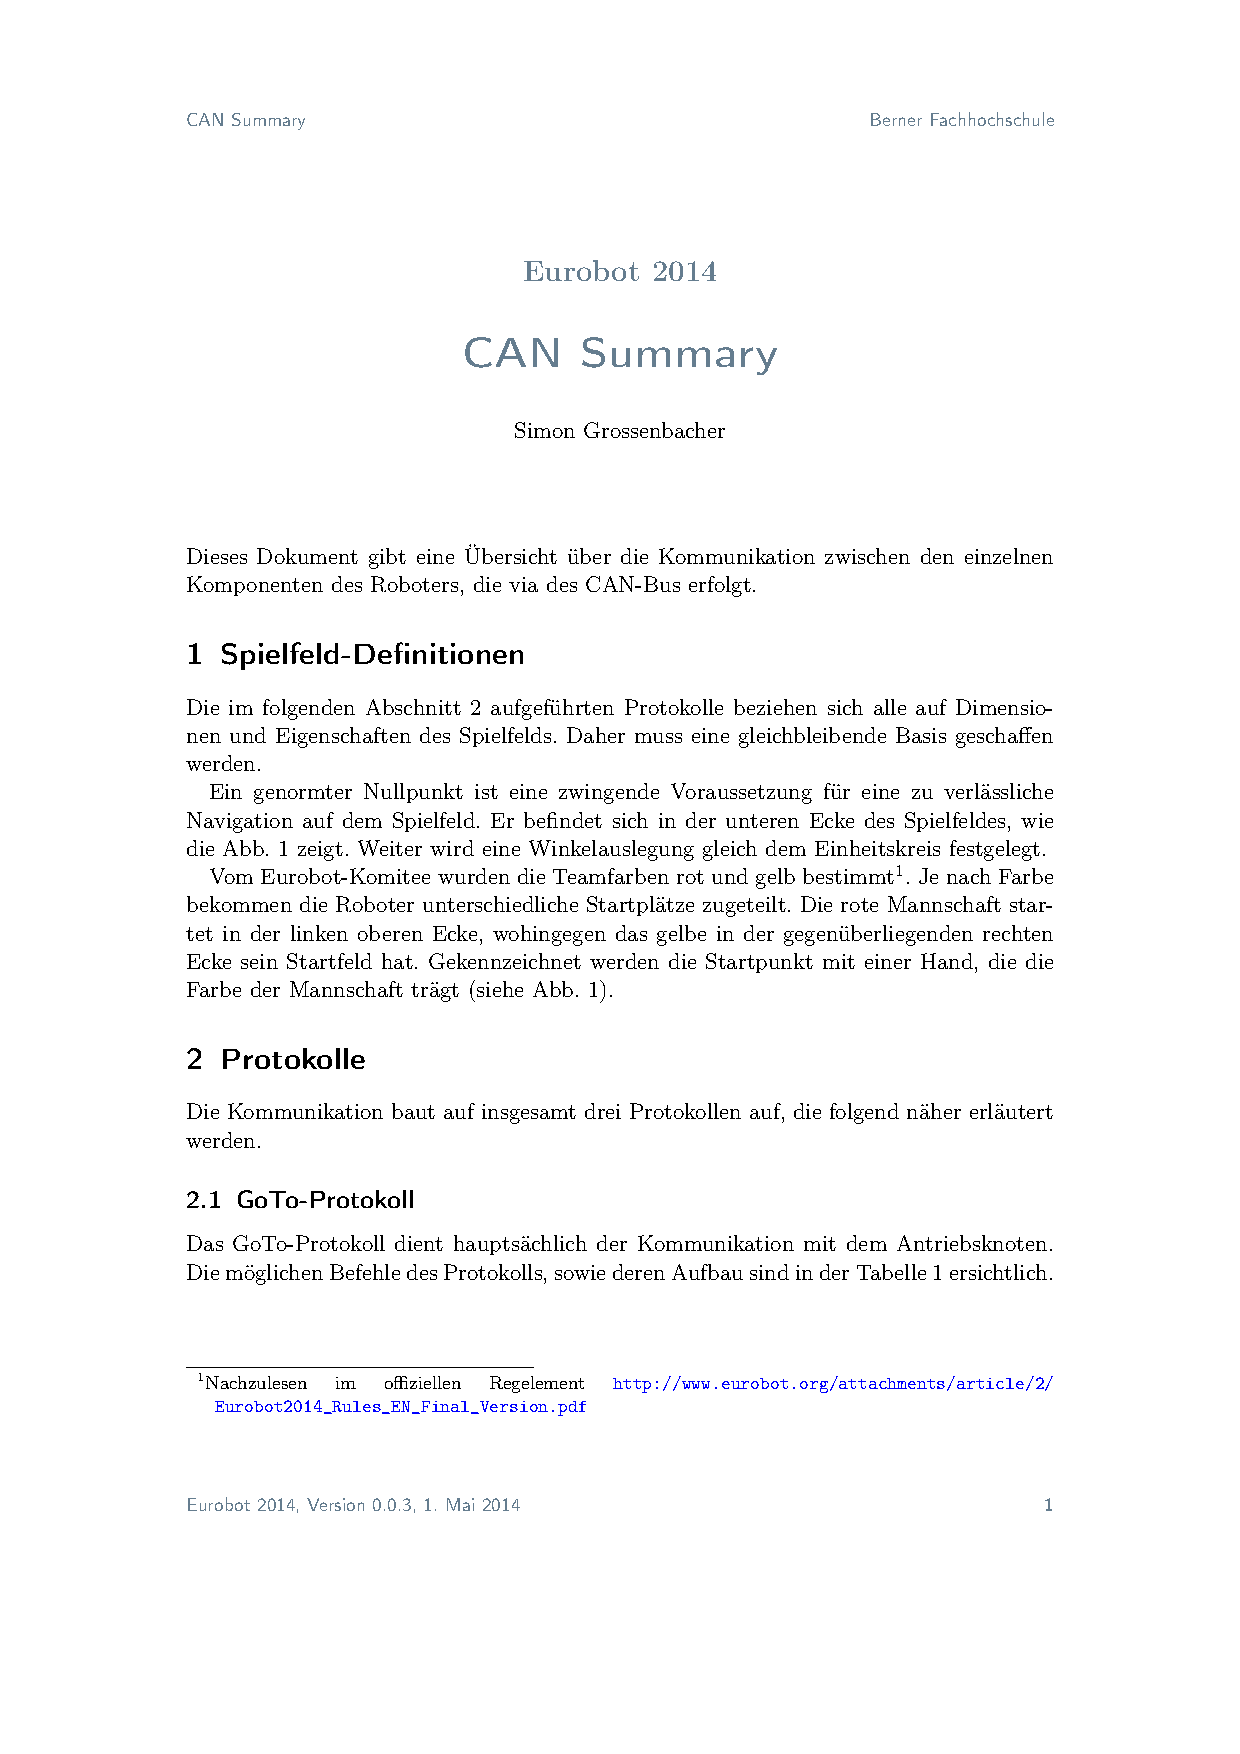
\includepdf[scale=0.8, pagecommand={}, pages=-, landscape=false]{appendix/image/i_can_summary_final.pdf}
%	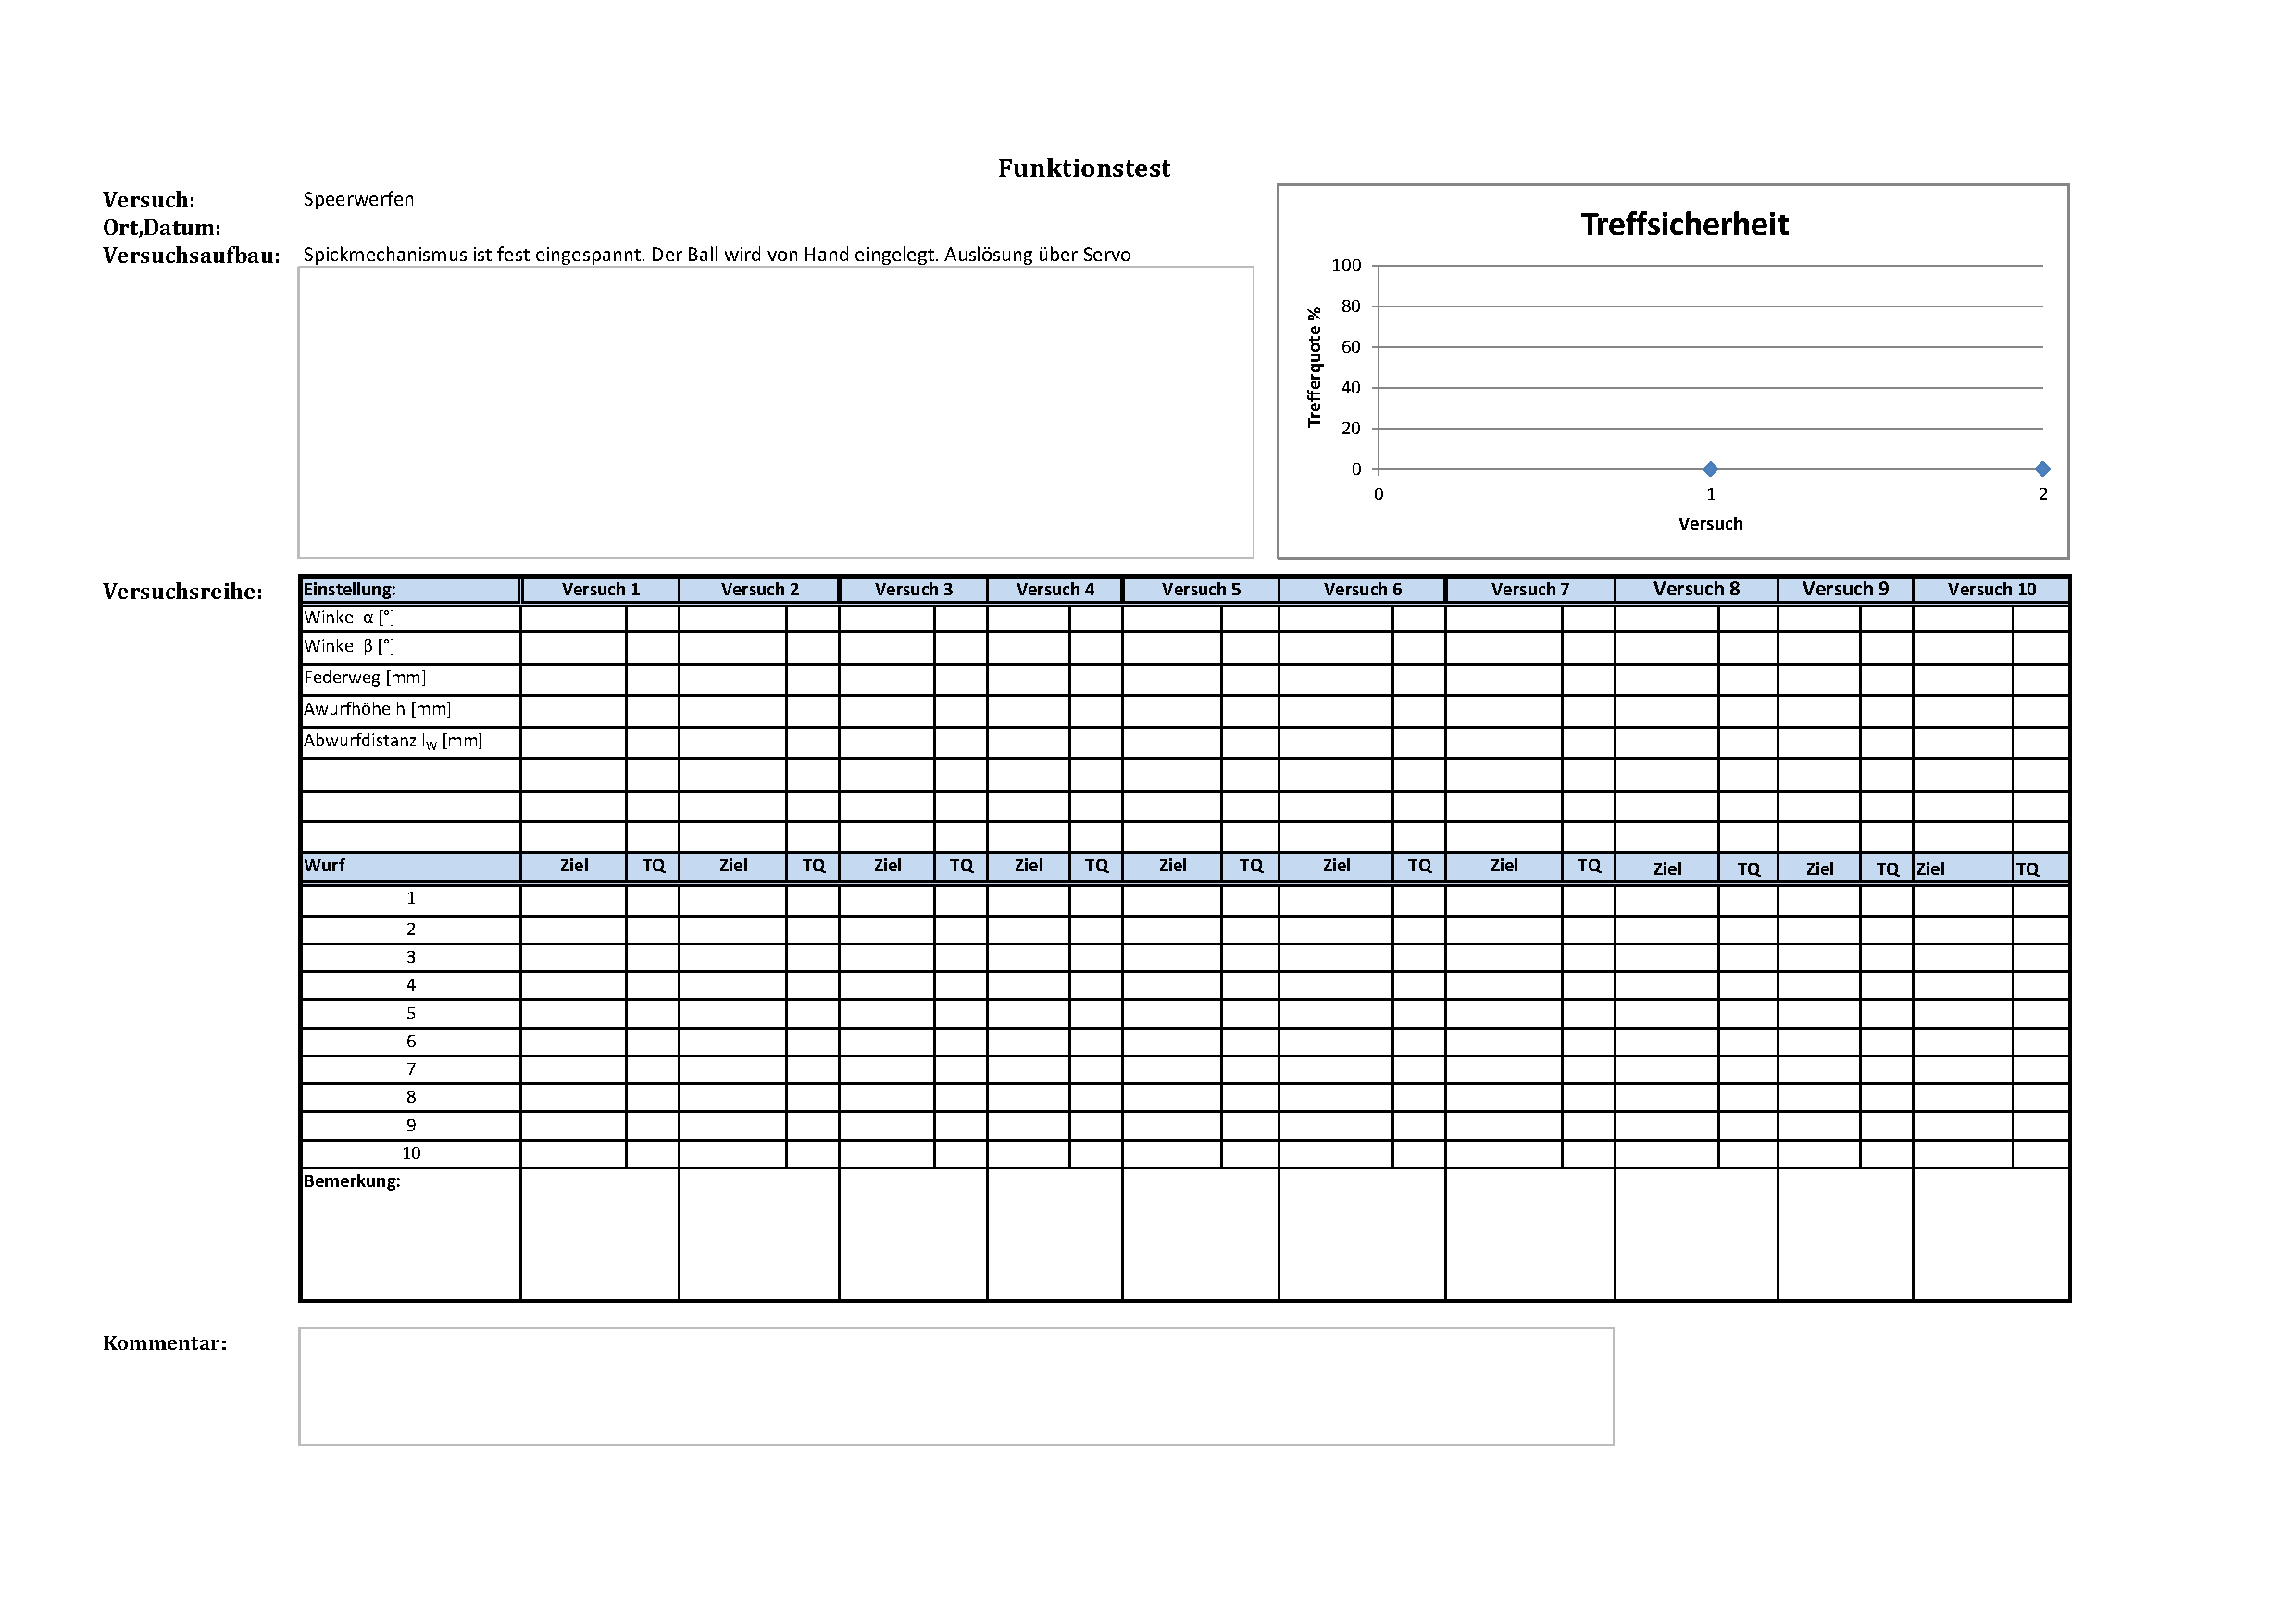
\includepdf[scale=0.7, pagecommand={\thispagestyle{plain}}, pages=-, landscape=true]{appendix/image/g_Funktionstest_Speerwerfen.pdf}
%	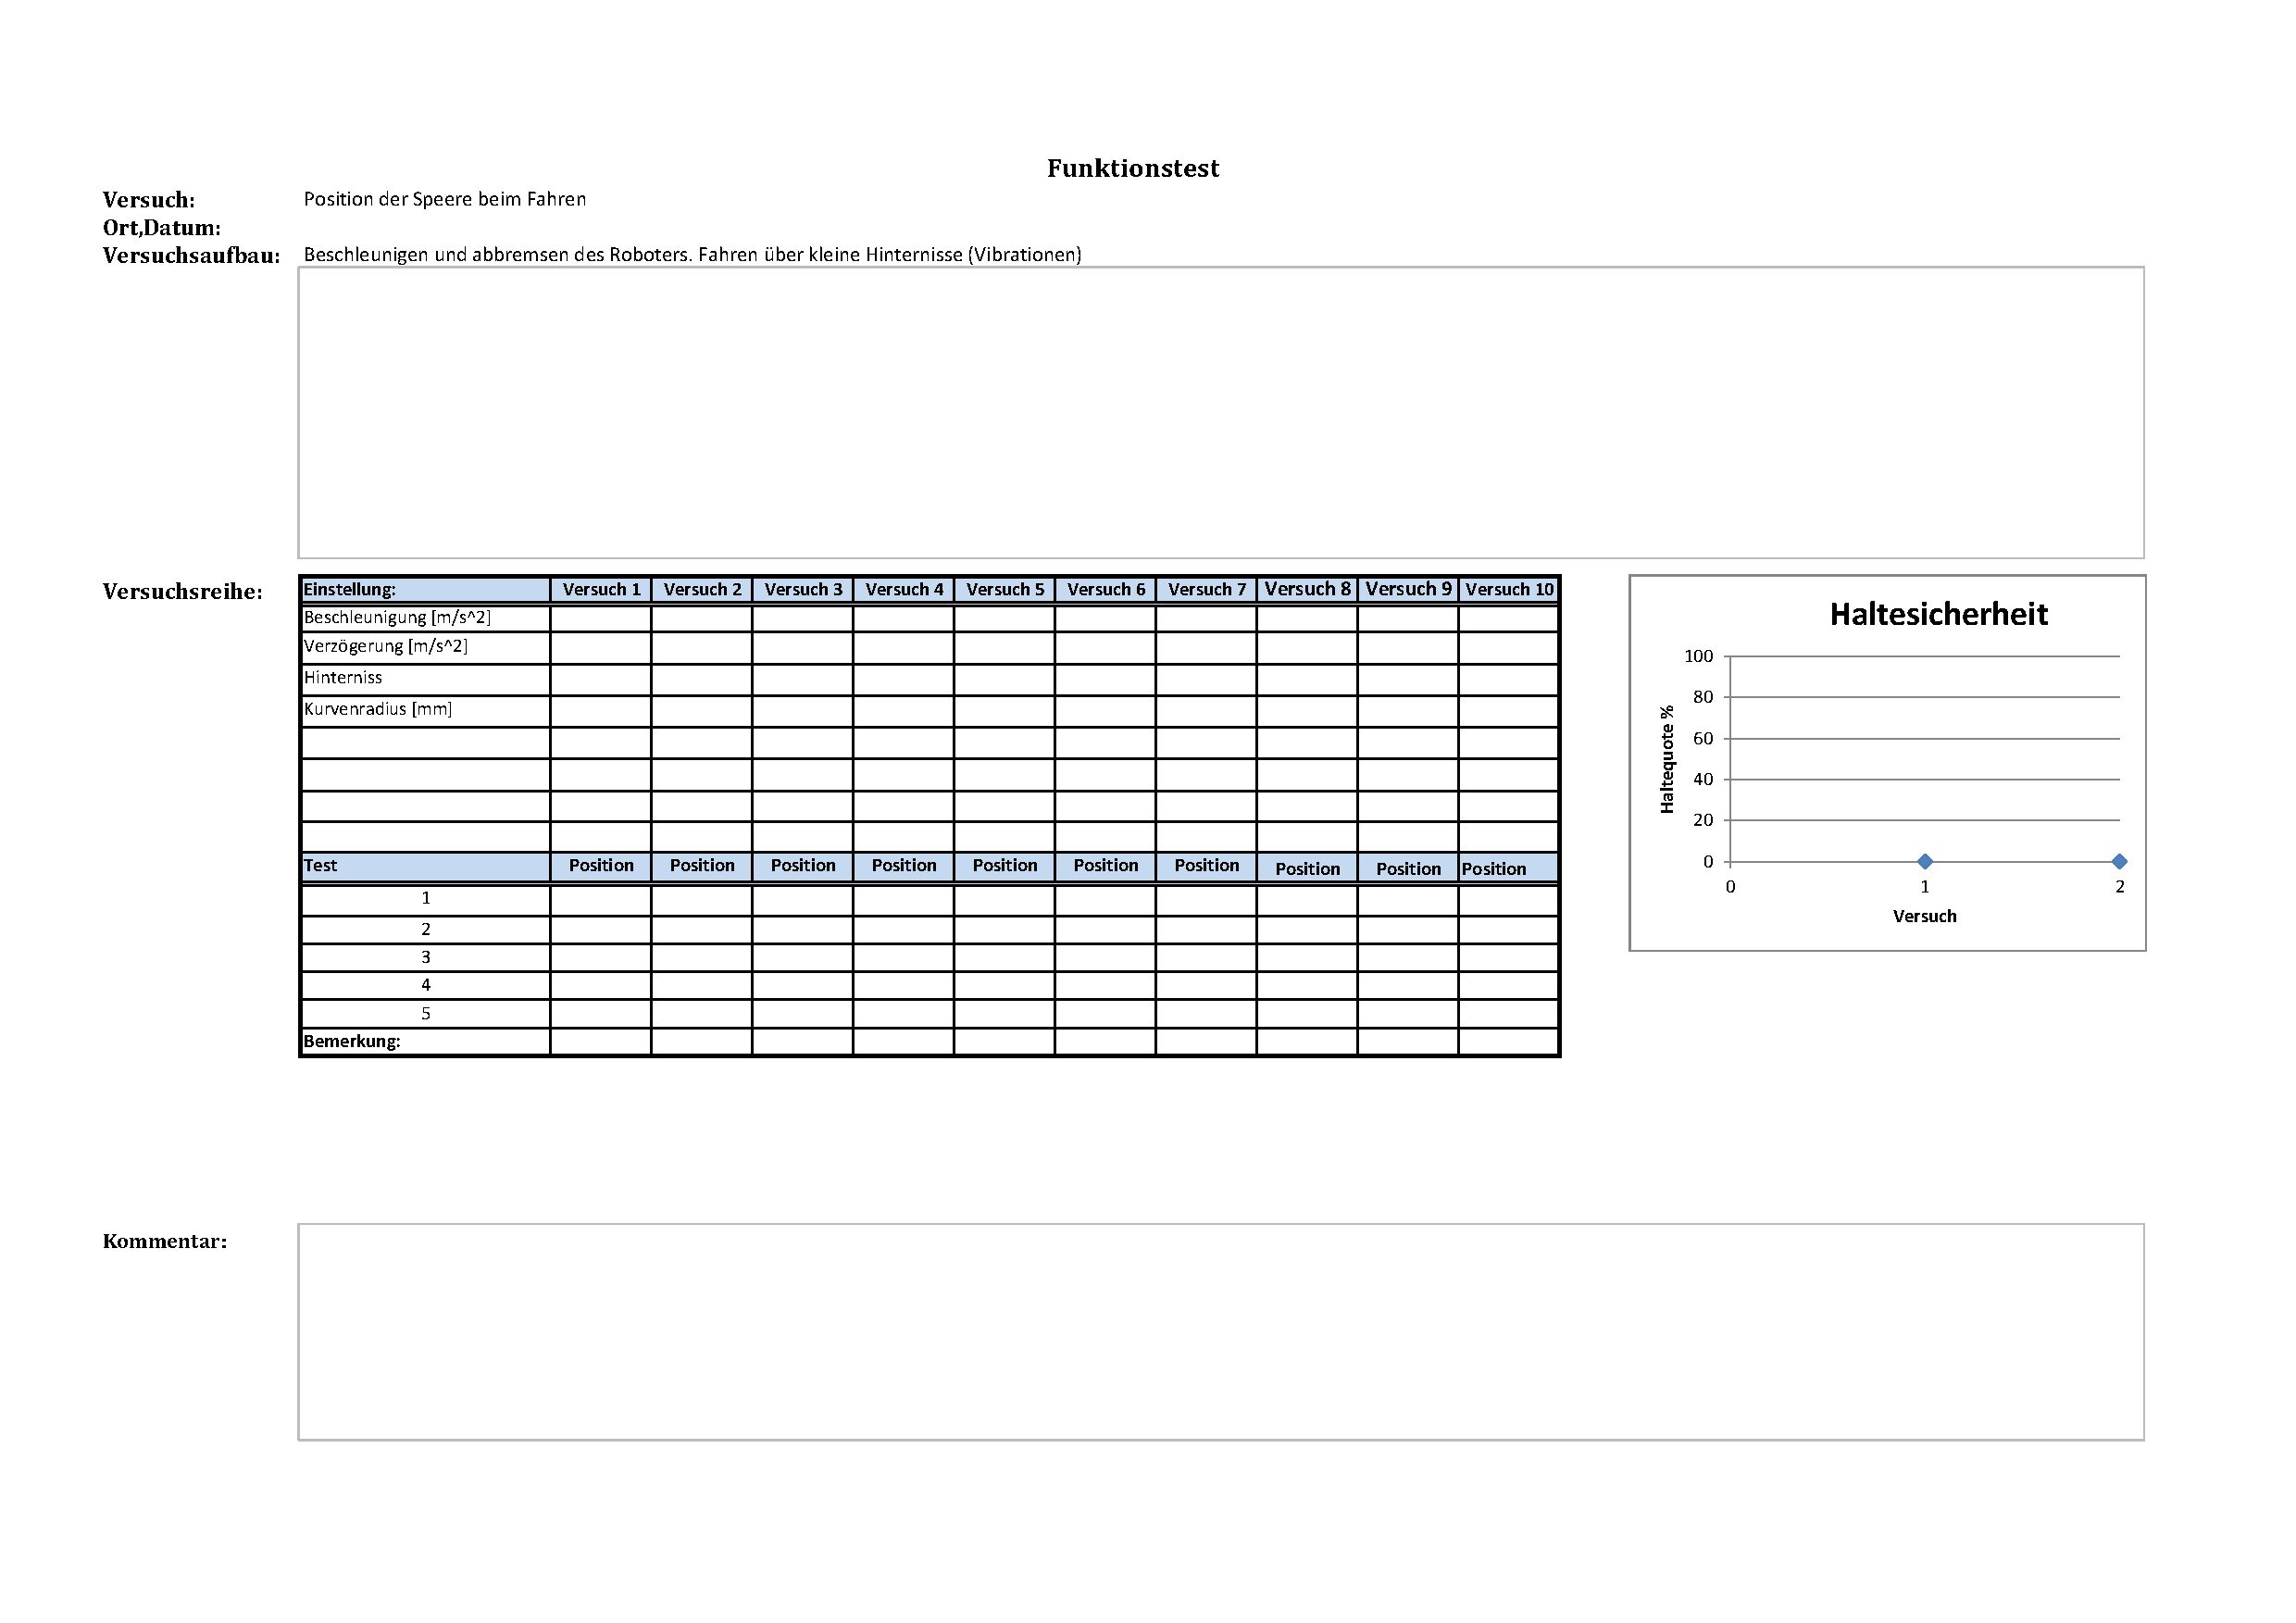
\includepdf[scale=0.7, pagecommand={\thispagestyle{plain}}, pages=-, landscape=true]{appendix/image/g_Funktionstest_Position_der_Speere_beim_Fahren.pdf}
    %
\includepdf[scale=0.85, pagecommand={\thispagestyle{plain}}, pages=-]{appendix/image/b_pflichtenheft.pdf}
    %
\includepdf[scale=0.85,pagecommand={\thispagestyle{plain}}, pages=-]{appendix/image/b_pflichtenheft.pdf}
